% $Id: views.tex 11058 2010-05-06 14:44:53Z alexandra $
% Local Variables:
% ispell-check-comments: nil
% Local IspellDict: american
% End:
% --------------------------------------------------------
% User documentation
% copyright by BREDEX GmbH 2004
% --------------------------------------------------------
\index{View}
\index{View!Editor}
\index{Editor!View}
\index{View!Test Result}
\index{Test!Result View}
\index{View!Properties}
\index{Properties View}
\index{View!Data Sets}
\index{Data Sets View}
\index{View!Problem}
\index{Problem View}
\index{Component!Names!View}
\index{View!Component Names}
\index{View!Search Result}
\index{Search Result View}
\index{View!Navigator}
\index{Navigator View}
\index{Console!View}
\index{View!Console}
\index{Test Result Summary View}
\index{View!Test Result Summary}
\index{View!Running AUT's}
\index{Running AUT's View}
\index{Inspector View}
\index{View!Inspector}
\index{View!Image}
\index{Image!View}

\app{} has the following views:

\begin{itemize}
\item \gdpropview{}
\item \gddatasetsview{}
\item \gdcompnamesview{}
\item \gdtestresultview{}
\item \gdprobview{}
\item Search result view
\item \gdnavview{}
\item Console
\item \gdinspector{}
\item \gdtestsummaryview{}
\item \gdrunautview{}
\item \gdimgview{}
\end{itemize}

The first three views are \emph{support views}. Their content changes depending on the current selection -- they show details corresponding to the currently selected item.

Use \bxmenu{Window}{Show View}{Other} to see a full list of views that can be opened in the \ite{}.
\subsection{The \gdpropview{}}
\gdhelpid{guidancerPropertiesViewContextId}{Properties View}

The \gdpropview{} is in the upper right-hand corner of each perspective. The \gdpropview{} shows details about the selected item in a browser or editor. 

If you select something from a browser, you can see its details in the \gdpropview{}, but you can't edit them. You can only edit details from within an editor. Read-only fields in the \gdpropview{} have a lock icon at their left-hand side. 
 \gdmarpar{../../../share/PS/readonly}{read only}

\textbf{\gdsuite{} details}

If you select a \gdsuite{}, you will see the following:
\begin{itemize}
\item The \gdsuite{} name.
\item Any comments for the \gdsuite{}. 
\item The step delay for this \gdsuite{}.
\item The name of the \gdaut{} this \gdsuite{} uses. 
\item The reentry properties for the default \gdehandlers{}. 
\end{itemize}

\textbf{\gdcase{} details}

If you select a \gdcase{}, the \gdpropview{} shows the following:

\begin{itemize}
\item The \gdcase{} name.
\item Any comments for the \gdcase{}. 
\item The data source details for this \gdcase{}
\item Any parameters/parameter values if references have been used in the \gdcase{}. 
\end{itemize}


\textbf{\gdstep{} details}

If you select a \gdstep{}, you will see the following:
\begin{itemize}
\item The \gdstep{} name.
\item Any comments for this \gdstep{}. 
\item Details about the component in the \gdstep{}:
\begin{itemize}
\item  The component type.
\item  The component name (given by you).
\end{itemize}
\item Details about the action in the \gdstep{}.
\item Details about the parameters in the \gdstep{}. For each parameter you will see:
\begin{itemize}
\item The parameter name.
\item The parameter type (e.g. if it is an integer, a string etc).
\item The parameter value (either a concrete value or a reference). 
\end{itemize}
\end{itemize}

\textbf{Test result details}

If you select an item from the \gdtestresultview{}, you will see the following:
\begin{itemize}
\item The result details:
\begin{itemize}
\item The name of the item.
\item What type of item it is.
\item Any comments for the item.
\end{itemize}
\item The test result -- if it passed or failed.
\item For \gdsteps{}, you can also see the component, action and parameter details. If the \gdstep{} failed, you can also see the error details. 
\item For \gdehandlers{}, you can see the type of \gdehandler{} it was, and what the reentry property was. 
\end{itemize}

 
\textbf{Icons in the \gdpropview{}}

When the \gdpropview{} contains data (i.e. a filled-in \emph{parameter value} field), there are certain icons to help you understand the data.  
\begin{itemize}
\item Values which are the same as in the original specification display 
a small gray diamond to the left of the field.
\gdmarpar{../../../share/PS/originalData}{original data}
\item Values which have been overwritten at a place of reuse show a small 
yellow diamond. 
\gdmarpar{../../../share/PS/overwrittenData}{overwritten data}
\end{itemize}


\subsection{The \gddatasetsview{}}
\gdhelpid{guidancerDataSetViewContextId}{Data Sets View}
The \gddatasetsview{} is in the lower right-hand corner of the \specpersp{}  by default. It lets you add, modify, delete and see any data for \gdcases{}. For each \gdcase{} containing references or for each central test data set, you can add data sets in this view. This is also the view where you can translate your data and overwrite data when you reuse a \gdcase{}. 
 When data in the \gddatasetsview are uneditable, they are shown in gray. Values in black may be edited.

To make entering data easier, pressing \bxkey{Enter} will spring to the next cell or row, or to the \bxcaption{Add} button if no more rows have been added. The \bxkey{Tab} key  springs to the \bxcaption{Add} button. 

\subsection{The \gdcompnamesview{}}
\gdhelpid{compNameViewContextId}{Component Names}
The \gdcompnamesview{} is in the lower right-hand corner of the \specpersp{}  by default, just behind the \gddatasetsview{}. It lets you see the component names used in a reused \gdcase{}, and add more component names. This means that you can use a \gdcase{} to execute the same actions on different components. 

\subsection{The \gdtestresultview{}} 
 \gdhelpid{testResultViewContextId}{Test Results View}

The \gdtestresultview{} is in the middle of the \execpersp{}  by default. It can also be displayed in the bottom right-hand corner of the \specpersp{} via the preferences. It follows and displays the results of the test execution. Each \gdstep{} and \gdcase{} is marked with a green tick or a red cross depending on if it passed or failed. 

If you select an item in the \gdtestresultview{}, you can see its details in the \gdpropview{}. If the \gdproject{} is open and the item is still available, you can double-click on a \gdstep{} or \gdcase{} in the \gdtestresultview{}, to highlight it in the \gdtestsuitebrowser{}. Double-clicking on this item in the \gdtestsuitebrowser{} will open the editor for this item in the \specpersp{}. 

\subsection{The \gdprobview{}}
\gdhelpid{problemViewContextId}{Problem View}
The \gdprobview{} is by default at the bottom of the \specpersp{}, under the editor area. The \gdpropview{} helps you to work with \app{} by giving you information, warnings and errors. Double-clicking on a message will either carry out the necessary action or open a dialog/editor to sort out the problem, if this is possible. 

\subsection{The search result view}
\gdhelpid{searchResultViewContextId}{Search Result View}
The search result view (\bxfigref{showresultview}) is at the bottom of the \specpersp{}, under the editor area, and just behind the \gdprobview{} by default. If you perform searches with \app{}, the results are shown here. If you double-click on an item in the search result view, the corresponding item is highlighted in the \gdtestcasebrowser{} or \gdtestsuitebrowser{}.  

\begin{figure}[hbtp]
\begin{center}
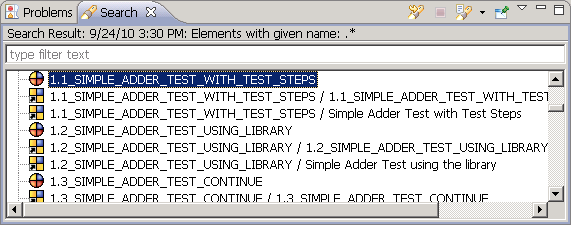
\includegraphics{Userinterface/Editors/PS/showresultview}
\caption{Search Result View}
\label{showresultview}
\end{center}
\end{figure}

\subsection{The \gdnavview{}}
\protect\gdhelpid{org.eclipse.ui.resource_view_context}{Navigator View}
The \gdnavview{} is at the top right-hand corner of the workspace perspective by default. The \gdnavview{} gives you a view of your workspace and the files in it. 


\subsection{The console}
The console is shown in the bottom right-hand corner of the \specpersp{}. It lets you follow certain processes in \app{}, for example, the import of \gdprojects{}.  

\subsection{The \gdinspector{}}
The \gdinspector{} can be used to help you test RCP \gdauts{} which use the GEF framework. When the inspector is activated, figures can be clicked in the GEF canvas, and their textpath (used to identify them in the test) is shown. The \gdinspector{} is shown by default in the bottom right-hand corner of the \specpersp{}. 

\subsection{The \gdtestsummaryview{}}
The \gdtestsummaryview{} offers an overview of all tests that have run in this \gddb{}. It can be filtered and sorted.  The \gdtestsummaryview{} is displayed in the \reportpersp{}. 

\subsection{The \gdrunautview{}}
The \gdrunautview{} is above the \gdtestsuitebrowser{} in the \specpersp{}. It shows an overview of all running \gdauts{} and can be used to stop \gdauts{} and to start \gdsuites{}.  

\subsection{The \gdimgview{}}
The \gdimgview{} is used to see automatically generated screenshots of errors that have occurred in tests.
